\section{Background}
\label{sec:background}

TODO: what shall we write here? about dependent types in general?

\section{Defining Agent-Based Simulation}
\label{sec:defining_abs}

Agent-Based Simulation (ABS) is a methodology to model and simulate a system where the global behaviour may be unknown but the behaviour and interactions of the parts making up the system is of knowledge. Those parts, called agents, are modelled and simulated out of which then the aggregate global behaviour of the whole system emerges. So the central aspect of ABS is the concept of an agent which can be understood as a metaphor for a pro-active unit, situated in an environment, able to spawn new agents and interacting with other agents in some neighbourhood by exchange of messages. 
We informally assume the following about our agents \cite{siebers_introduction_2008}, \cite{wooldridge_introduction_2009}, \cite{siebers_discrete-event_2010}, \cite{dawson_opening_2014}, \cite{macal_everything_2016}:

\begin{itemize}
	\item They are uniquely addressable entities with some internal state over which they have full, exclusive control.
	\item They are pro-active which means they can initiate actions on their own e.g. change their internal state, send messages, create new agents, terminate themselves.
	\item They are situated in an environment and can interact with it.
	\item They can interact with other agents which are situated in the same environment by means of messaging.
\end{itemize} 

\begin{comment}
Epstein \cite{epstein_generative_2012} identifies ABS to be especially applicable for analysing \textit{"spatially distributed systems of heterogeneous autonomous actors with bounded information and computing capacity"}. %Thus in the line of the established simulation methodologies (see Table \ref{tab:simulation_types}), ABS is the most powerful one as listed in :
It exhibits the following properties:

\begin{itemize}
	\item Linearity \& Non-Linearity - actions of agents can lead to non-linear behaviour of the system.
	\item Time - agents act over time which is also the source of their pro-activity.
	\item States - agents encapsulate some state which can be accessed and changed during the simulation.
	\item Feedback-Loops - because agents act continuously and their actions influence each other and themselves in subsequent time-steps, feedback-loops are the norm in ABS. 
	\item Heterogeneity - although agents can have same properties like height, sex,... the actual values can vary arbitrarily between agents.
	\item Interactions - agents can be modelled after interactions with an environment or other agents. %, making this a unique feature of ABS, not possible in the other simulation models.
	\item Spatiality \& Networks - agents can be situated within e.g. a spatial (discrete 2D, continuous 3D,...) or complex network environment. % making this also a unique feature of ABS, not possible in the other simulation models.
\end{itemize}
\end{comment}

\begin{comment}
Note that there doesn't exist a commonly agreed technical definition of ABS but the field draws inspiration from the closely related field of Multi-Agent Systems (MAS) \cite{wooldridge_introduction_2009}, \cite{weiss_multiagent_2013}. It is important to understand that MAS and ABS are two different fields where in MAS the focus is much more on technical details, implementing a system of interacting intelligent agents within a highly complex environment with the focus primarily on solving AI problems.
\end{comment}

\section{Case Study I: SIR}
\label{sec:concurrent_sir}
Our first case study is the SIR model as introduced in Chapter \ref{sec:sir_model}. The aim of this case study is to investigate the potential speed up a concurrent \textit{STM} implementation gains over a sequential one under varying number of CPU cores and agents. The behaviour of the agents is quite simple and the interactions are happening indirectly through the environment, where reads from the environment outnumber the writes to it by far. Further, a comparison to a lock-based implementation with the \textit{IO} Monad is done to understand that \textit{STM} is also able to outperform traditional concurrency, \textit{in a pure functional ABS setting} while still retaining its greater static guarantees than \textit{IO} \footnote{The code of all three implementations is available at \url{https://github.com/thalerjonathan/phd/tree/master/public/stmabs/code/SIR}}.

\begin{enumerate}
	\item Sequential - this is the original implementation as discussed in Chapter \ref{sec:adding_env}, where the discrete 2D environment is shared amongst all agents as read-only data and the agents are executed sequentially within the main thread without any concurrency.
	\item STM - this is the same implementation as the \textit{Sequential} one but agents run now in the \textit{STM} Monad and have access to the discrete 2D environment through a transactional variable \textit{TVar}. This means that the agents now communicate indirectly by reads and writes through the \textit{TVar}.
	\item Lock-Based - this follows the \textit{STM} implementation, with the agents running in \textit{IO}. They share the discrete 2D environment using an \textit{IORef} and have access to an \textit{MVar} lock to synchronise access to it.
\end{enumerate}

Each experiment was run until $t = 100$ and stepped using $\Delta t = 0.1$. For each experiment we conducted 8 runs on our machine (see Table \ref{tab:machine_specs}) under no additional work-load and report the mean. %Further, we checked the visual outputs and the dynamics and they look qualitatively the same as the reference \textit{Sequential}. We could have used more rigour and properly validated the implementations against the formal specification using tests as we do in Chapter Property-based testing but we leave this for further res.
In the experiments we varied the number of agents (grid size) as well as the number of cores when running concurrently - the numbers are always indicated clearly.

\begin{table}
	\centering
	\begin{tabular}{ c || c }
		OS & Fedora 28, 64-bit \\ \hline
		RAM & 16 GByte \\ \hline
		CPU & Intel i5-4670K @ 3.4GHz \\ \hline
		HD & 250Gbyte SSD \\ \hline
		Haskell & GHC 8.2.2
	\end{tabular}
	
	\caption{Machine and Software specs for all experiments}
	\label{tab:machine_specs}
\end{table}

\subsection{Constant Grid Size, Varying Cores}
In this experiment we held the grid size constant to 51 x 51 (2,601 agents) and varied the cores. The results are reported in Table \ref{tab:constgrid_varyingcores}.

\begin{table}
	\centering
	\begin{tabular}{cc|c}
		\multicolumn{1}{ c||  }{\multirow{2}{*}{} } &
		\multicolumn{1}{ |c| }{Cores} & Duration      \\ \hline \hline 
		
		\multicolumn{1}{ c||  }{\multirow{1}{*}{Sequential} } &
		\multicolumn{1}{ |c| }{1} & 72.5      \\ \hline \hline 
		
		\multicolumn{1}{ c||  }{\multirow{4}{*}{Lock-Based} } &
		\multicolumn{1}{ |c| }{1} & 60.6       \\ \cline{2-3}
		\multicolumn{1}{ c||  }{}                       &
		\multicolumn{1}{ |c| }{2} & 42.8    \\ \cline{2-3}
		\multicolumn{1}{ c||  }{}                       &
		\multicolumn{1}{ |c| }{3} & 38.6    \\ \cline{2-3}
		\multicolumn{1}{ c||  }{}                       &
		\multicolumn{1}{ |c| }{4} & 41.6    \\ \hline \hline 
		
		\multicolumn{1}{ c||  }{\multirow{4}{*}{STM} } &
		\multicolumn{1}{ |c| }{1} & 53.2       \\ \cline{2-3}
		\multicolumn{1}{ c||  }{}                       &
		\multicolumn{1}{ |c| }{2} & 27.8    \\ \cline{2-3}
		\multicolumn{1}{ c||  }{}                       &
		\multicolumn{1}{ |c| }{3} & 21.8    \\ \cline{2-3}
		\multicolumn{1}{ c||  }{}                       &
		\multicolumn{1}{ |c| }{4} & \textbf{20.8}    \\ \hline \hline 
	\end{tabular}
  	
  	\caption{Experiments on 51x51 (2,601 agents) grid with varying number of cores. Timings in seconds (lower is better).}
	\label{tab:constgrid_varyingcores}
\end{table}

The \textit{STM} implementation running on 4 cores shows a speed up factor of 3.6 over \textit{Sequential}, which is a quite impressive number when considering that we can achieve at most a factor of 4 when running on 4 cores. It seems that \textit{STM} allow us to push the practical limit very close to the theoretical one, whereas the \textit{Lock-Based} approach just arrives at a factor of 1.74 on 4 cores.

Comparing the performance and scaling to multiple cores shows that the \textit{STM} implementation significantly outperforms the \textit{Lock-Based} one and scales better to multiple cores. The \textit{Lock-Based} implementation performs best with 3 cores and shows slightly worse performance on 4 cores as can be seen in Figure \ref{fig:core_duration_stm_io}. This is no surprise because the more cores are running at the same time, the more contention for the lock, thus the more likely synchronisation happening, resulting in higher potential for reduced performance. This is not an issue in \textit{STM} because no locks are taken in advance. 

\begin{figure}
	\centering
	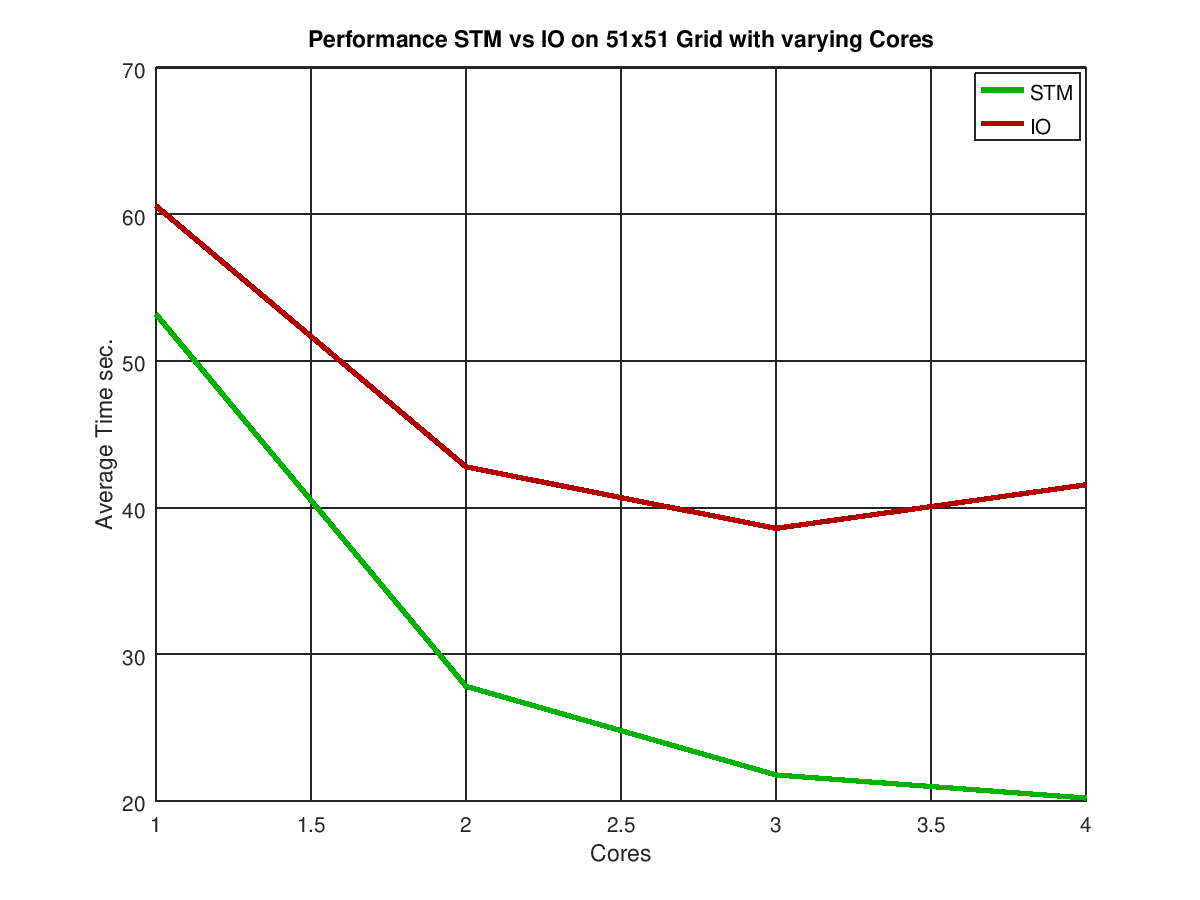
\includegraphics[width=0.8\textwidth, angle=0]{./fig/concurrentabs/sir/core_duration_stm_io.png}
	\caption{Comparison of performance and scaling on multiple cores of STM and Lock-Based. Note that the Lock-Based implementation seems to perform slightly worse on 4 than on 3 cores probably due to lock-contention.}
	\label{fig:core_duration_stm_io}
\end{figure}

\subsection{Varying Grid Size, Constant Cores}
In this experiment we varied the grid size and used always 4 cores. The results are reported in Table \ref{tab:varyinggrid_constcores} and plotted in Figure \ref{fig:varyinggrid_constcores}.

\begin{table}
	\centering
  	\begin{tabular}{ c || c | c | c }
        Grid-Size          & STM              & Lock-Based   & Ratio \\ \hline \hline 
   		51 x 51 (2,601)    & \textbf{20.2}    & 41.9         & 2.1 \\ \hline
   		101 x 101 (10,201) & \textbf{74.5}    & 170.5        & 2.3 \\ \hline
   		151 x 151 (22,801) & \textbf{168.5}   & 376.9        & 2.2 \\ \hline
   		201 x 201 (40,401) & \textbf{302.4}   & 672.0        & 2.2 \\ \hline
   		251 x 251 (63,001) & \textbf{495.7}   & 1,027.3      & 2.1 \\ \hline \hline
  	\end{tabular}

  	\caption{Performance on varying grid sizes. Timings in seconds (lower is better). Ratio compares STM to Lock-Based.}
	\label{tab:varyinggrid_constcores}
\end{table}

It is clear that the \textit{STM} implementation outperforms the \textit{Lock-Based} implementation by a substantial factor.

\begin{figure}
	\centering
	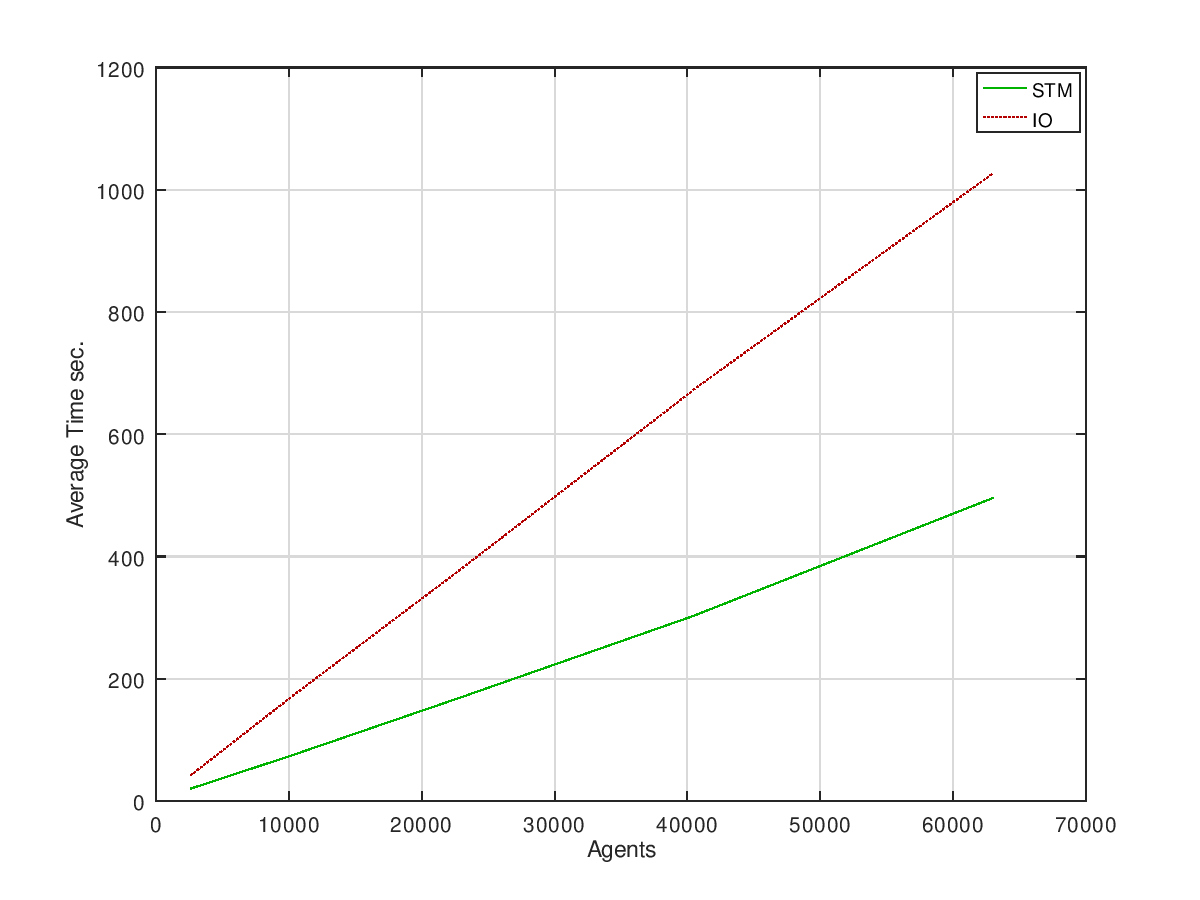
\includegraphics[width=1\textwidth, angle=0]{./fig/concurrentabs/sir/stm_io_varyinggrid_performance.png}
	\caption{Performance on varying grid sizes.}
	\label{fig:varyinggrid_constcores}
\end{figure}

\subsection{Retries}
Of very much interest when using STM is the retry-ratio, which obviously depends highly on the read-write patterns of the respective model. We used the \textit{stm-stats} library to record statistics of commits, retries and the ratio. The results are reported in Table \ref{tab:retries_stm}.

\begin{table}
	\centering
  	\begin{tabular}{ c || c | c | c }
        Grid-Size 		   & Commits    & Retries & Ratio \\ \hline \hline 
   		51 x 51 (2,601)    & 2,601,000  & 1306.5  & 0.0 \\ \hline
   		101 x 101 (10,201) & 10,201,000 & 3712.5  & 0.0 \\ \hline
   		151 x 151 (22,801) & 22,801,000 & 8189.5  & 0.0 \\ \hline
   		201 x 201 (40,401) & 40,401,000 & 13285.0 & 0.0 \\ \hline 
   		251 x 251 (63,001) & 63,001,000 & 21217.0 & 0.0 \\ \hline \hline
  	\end{tabular}
  	
  	\caption{Retry ratios on varying grid sizes on 4 cores.}
	\label{tab:retries_stm}
\end{table}

Independent of the number of agents we always have a retry-ratio of 0.0. This indicates that this model is \textit{very} well suited to STM, which is also directly reflected in the much better performance over the \textit{Lock-Based} implementation. Obviously this ratio stems from the fact that in our implementation we have \textit{very} few writes, which happen only in case when an agent changes from Susceptible to Infected or from Infected to Recovered. On the other hand, there are a very large number of reads due to indirect agent interaction. For \textit{STM} this is no problem because no lock is taken but the \textit{Lock-Based} approach is forced to conservatively take the lock to ensure mutual exclusive access to the critical section across all agents.

\subsection{Going Large-Scale}
To test how far we can scale up the number of cores in both the \textit{Lock-Based} and \textit{STM} cases, we ran two experiments, 51x51 and 251x251, on Amazon EC2 instances with a larger number of cores than our local machinery, starting with 16 and 32 to see if we are running into decreasing returns. The results are reported in Table \ref{tab:sir_varying_cores_amazon}.

\begin{table}
	\centering
  	\begin{tabular}{cc|c|c}
		\multicolumn{1}{ c||  }{\multirow{2}{*}{} } &
		\multicolumn{1}{ |c| }{Cores} & 51x51    & 251x251       \\ \hline \hline 
		
		\multicolumn{1}{ c||  }{\multirow{2}{*}{Lock-Based} } &
		\multicolumn{1}{ |c| }{16} & 72.5    & 1830.5       \\ \cline{2-4}
		\multicolumn{1}{ c||  }{}                       &
		\multicolumn{1}{ |c| }{32} & 73.1    & 1882.2      \\ \hline \hline 
		
		\multicolumn{1}{ c||  }{\multirow{2}{*}{STM} } &
		\multicolumn{1}{ |c| }{16} & \textbf{8.6}     & \textbf{237.0}       \\ \cline{2-4}
		\multicolumn{1}{ c||  }{}                       &
		\multicolumn{1}{ |c| }{32} & 12.0    & 248.7      \\ \hline \hline 
	\end{tabular}

  	\caption{Performance on varying cores on Amazon S2 Services. Timings in seconds (lower is better).}
	\label{tab:sir_varying_cores_amazon}
\end{table}

As expected, the \textit{Lock-Based} approach doesn't scale up to many cores because each additional core brings more contention to the lock, resulting in an even more decreased performance, even worse than the \textit{Sequential} implementation. This is particularly obvious in the 251x251 experiment because of the much larger number of concurrent agents. The \textit{STM} approach returns better performance on 16 cores but fails to scale further up to 32 where the performance drops below the one with 16 cores. In both STM cases we measured a retry-ratio of 0, thus we assume that with 32 cores we become limited by the overhead of STM transactions \cite{perfumo_limits_2008} because the workload of an STM action in our SIR implementation is quite small.

Compared to the \textit{Sequential} implementation, \textit{STM} reaches a speed up factor of 8.4 on 16 cores, which is still impressive but is much further away from the theoretical limit than in the case of only 4 cores -  a further indication that this model in particular and our approach in general does not scale up arbitrarily.

% NOTE: 0 retries in both cases means that the STM transactions themselves are becoming the bottleneck. this makes sens because the STM trasnactions in our SIR implementation are very small (especially recovered and infected agent) and could therefore really cause substantial overhead as pointed out by \cite{perfumo_limits_2008}
%16 cores 251x251: 0.0 retry-ratio
%32 cores 251x251: 0.0 retry ratio
%
%16 cores 51x51: 0.0 retry-ratio
%32 cores 51x51: 0.0 retry ratio

\subsection{Discussion}
The timing measurements speak a clear language: running in \textit{STM} and sharing state using a transactional variable \textit{TVar} is much more time-efficient than both the \textit{Sequential} and \textit{Lock-Based} approach. On 4 cores \textit{STM} achieves a speed up factor of 3.6, nearly reaching the theoretical limit.
Obviously both \textit{STM} and \textit{Lock-Based} sacrifices determinism: repeated runs might not lead to same dynamics despite same initial conditions. Still, by sticking to \textit{STM}, we get the guarantee that the source of this non-determinism is concurrency within the \textit{STM} monad but \textit{nothing else}. This we can not guarantee in the case of the \textit{Lock-Based} approach as all bets are off when running within \textit{IO}. The fact to have \textit{both} the better performance \textit{and} the stronger static guarantees in the \textit{STM} approach makes it \textit{very} compelling.

\subsection{Sugarscape}
TODO

Sugarscape is an exploratory model inspired by real-world phenomenon which means it has lots of hypotheses implicit in the model but there does not exist real-world data / dynamics against which one could validate the simulated dynamics. Still we can conduct black-box verification because we have an informal model specification but we cannot do any statistical testing of simulated dynamics as we don't have data acting as ground-truth. But what we can do and what we will explore extensively in this section is how we can encode hypotheses about the dynamics (prior to running the simulation) in unit- and property-based tests and check them. Obviously white-box verification applies as well because we can reason about the code whether it matches the informal model specification or not.

\subsection{Verification \& Validation in ABS}
TODO

Validation \& Verification in ABS
\url{http://www2.econ.iastate.edu/tesfatsi/VVAccreditationSimModels.OBalci1998.pdf} : verification = are we building the model right? validation = are we building the right model?

good paper \url{http://www2.econ.iastate.edu/tesfatsi/VVAccreditationSimModels.OBalci1998.pdf} : very nice 15 guidelines and life cycles, VERY valuable for background and introduction

\url{http://www2.econ.iastate.edu/tesfatsi/VVSimulationModels.JKleijnen1995.pdf} : suggests good programming practice which is extremely important for high quality code and reduces bugs but real world practice and experience shows that this alone is not enough, even the best programmers make mistakes which often can be prevented through a strong static or a dependent type system already at compile time. What we can guarantee already at compile time, doesn't need to be checked at run-time which saves substantial amount of time as at run-time there may be a huge number of execution paths through the simulation which is almost always simply not feasible to check (note that we also need to check all combinations). This paper also cites modularity as very important for verification: divide and conquer and test all modules separately. this is especially easy in functional programming as composability is much better than with traditional oop due to the lack of interdependence between data and code as in objects and the lack of global mutable state (e.g. class variables or global variables) - this makes code extremely convenient to test. The paper also discusses statistical tests (the t test) to check if the outcome of a simulation is sufficiently close to real-world dynamics. Also the paper suggests using animations to visualise the processes within the simulation for verification purposes (of course they note that animation may be misleading when one focuses on too short simulation runs).

good paper:\url{ https://link.springer.com/chapter/10.1007/978-3-642-01109-2_10}
	-> verification. "This is essentially the question: does the model do what we think it is supposed to do? Whenever a model has an analytical solution, a condition which embraces almost all conventional economic theory, verification is a matter of checking the mathematics."
	-> validation: "In an important sense, the current process of building ABMs is a discovery process, of discovering the types of behavioural rules for agents which appear to be consistent with phenomena we observe."
		=> can we encode phenomena we observe in the types? can we use types for the discovery process as well? can dependent types guide our exploratory approach to ABS?
	-> "Because such models are based on simulation, the lack of an analytical solution (in
general) means that verification is harder, since there is no single result the model
must match. Moreover, testing the range of model outcomes provides a test only in
respect to a prior judgment on the plausibility of the potential range of outcomes.
In this sense, verification blends into validation."

either one has an analytical model as the basis of an agent-based model (ABM) or one does not.
In the former case, e.g. the SIR model, one can very easily validate the dynamcis generated by the ABM to the one generated by the analytical solution (e.g. through System Dynamics). Of course the dynamics wont be exactly the same as ABS discretisizes the approach and introduces stochastics which means, one must validate averaged dynamics.
In the latter case one has basically no idea or description of the emergent behaviour of the system prior to its execution. It is important to have some hypothesis about the emergent property / dynamics. The question is how verification / validation works in this setting as there is no formal description of the expected behaviour: we don't have a ground-truth against which we can compare our simulation dynamics. (eventuell hilft hier hans vollbrecht weiter: Simulation hat hier den Sinn, die Controller anhand der Roboteraufgabe zu validieren, Bei solchen Simulationen ist man interessiert an allen möglichen Sequenzen, und da das meist zu viele sind, an einer möglichst gut verteilten Stichprobenmenge. Hier geht es weniger um richtige Zeitmodellierung, sondern um den Test aller möglichen Ereignissequenzen.)

look into DEVS

TODO: the implementation phase is just one stage in a longer process \url{http://jasss.soc.surrey.ac.uk/12/1/1.html}

WE FOCUS ON VERIFICATION
important: we are not concerned here with validating a model with the real world system it simulates. this is an entirely different problem and focuses on the questions if we have built the right model.
we are interested here in extremely strong verification: have we built the model right? we are especially interested in to which extend purely and dependently-typed functional programming can support us in this task.

\url{http://jasss.soc.surrey.ac.uk/8/1/5.html}: "For some time now, Agent Based Modelling has been used to simulate and explore complex systems, which have proved intractable to other modelling approaches such as mathematical modelling. More generally, computer modelling offers a greater flexibility and scope to represent phenomena that do not naturally translate into an analytical framework. Agent Based Models however, by their very nature, require more rigorous programming standards than other computer simulations. This is because researchers are cued to expect the unexpected in the output of their simulations: they are looking for the 'surprise' that shows an interesting emergent effect in the complex system. It is important, then, to be absolutely clear that the model running in the computer is behaving exactly as specified in the design. It is very easy, in the several thousand lines of code that are involved in programming an Agent Based Model, for bugs to creep in. Unlike mathematical models, where the derivations are open to scrutiny in the publication of the work, the code used for an Agent Based Model is not checked as part of the peer-review process, and there may even be Intellectual Property Rights issues with providing the source code in an accompanying web page."

\url{http://jasss.soc.surrey.ac.uk/12/1/1.html}: "a prerequisite to understanding a simulation is to make sure that there is no significant disparity between what we think the computer code is doing and what is actually doing. One could be tempted to think that, given that the code has been programmed by someone, surely there is always at least one person - the programmer - who knows precisely what the code does. Unfortunately, the truth tends to be quite different, as the leading figures in the field report, including the following: You should assume that, no matter how carefully you have designed and built your simulation, it will contain bugs (code that does something different to what you wanted and expected), "Achieving internal validity is harder than it might seem. The problem is knowing whether an unexpected result is a reflection of a mistake in the programming, or a surprising consequence of the model itself. […] As is often the case, confirming that the model was correctly programmed was substantially more work than programming the model in the first place. This problem is particularly acute in the case of agent-based simulation. The complex and exploratory nature of most agent-based models implies that, before running a model, there is some uncertainty about what the model will produce. Not knowing a priori what to expect makes it difficult to discern whether an unexpected outcome has been generated as a legitimate result of the assumptions embedded in the model or, on the contrary, it is due to an error or an artefact created in the model design, its implementation, or its execution."


general requirements to ABS
- modelling progress of time (steward robinson simulation book, chapter 2)
- modelling variability (steward robinson simulation book, chapter 2)
- fixing random number streams to allow simulations to be repeated under same conditions (steward robinson simulation book, chapter 1.3.2 and chapter 2)
- only rely on past
	-> solved with Arrowized FRP
- bugs due to implicitly mutable state
	-> can be ensured by pure functional programming
- ruling out external sources of non-determinism / randomness
	-> can be ensured by pure functional programming
- correct interaction protocols
	-> can be ensured by dependent state machines
- deterministic time-delta
	-> TODO: can we ensure it through dependent-types at type-level?
- repeated runs lead to same dynamics
	-> can be ensured by pure functional programming

steward robinson simulation book bulletpoints
- chapter 8.2: speed of coding, transparency, flexibility, run-speed
- chapter 8.3: three activities - 1 coding, 2 testing verification and white-box validating, 3 documenting
- chapter 9.7: nature of simulation: terminating vs. non-terminating
- chapter 9.7: nature of simulation output: transient or steady-state (steady-state cycle, shifting steady-state)

steward robinson simulation book on implementation
- meaning of implementation
	-> 1 implementing the findings: conduct a study which defines and gathers all findings about the model and document them
	-> 2 implementing the model
	-> 3 implementing the learning

steward robinson simulation book on verification, validation and confidence
- Verification is the process of ensuring that the model design has been transformed into a computer model with sufficient accuracy (Davis 1992)
- Validation is the process of ensuring that the model is sufficiently accurate for the purpose at hand (Carson 1986).
- Verification has a narrow definition and can be seen as a subset of the wider issue of validation
- In Verification and validation the aim is to ensure, that the model is sufficiently accurate, which always implies its purpose.
- => the purpose / objectives mus be known BEFORE it is validated 
- white-box validation: detailed, micro check if each part of the model represent the real world with sufficient accuracy 
	-> intrinsic to model coding
- black-box validation: overall, macro check whether the model provides a sufficiently accurate representation of the real world system
	-> can only be performed once model code is complete
- other definition of verification: it is a test of the fidelity with which the conceptual model is converted into the computer model
- verification (and validation) is a continuous process => if it is already there in the programming language / supported by it e.g. through types,... then this is much easier to do
- difficulties of verification and validation
	-> there is no such thing as general validity: a model should be built for one purpose as simple as possible and not be too general, otherwise it becomes too bloated and too difficult / impossible to analyse
	-> there may be no real world to compare against: simulations are developed for proposed systems, new production / facilities which dont exist yet. 
	-> which real world?: the real world can be interpreted in different ways => a model valid to one person may not be valid to another
	-> often the real world data are inaccurate
	-> there is not enough time to verify and validate everything
	-> confidence, not validity: it is not possible to prove that a model is valid, instead one should think of confidence in its validity. 
		=> verification and validation is thus not the proof that a model is correct but trying to prove that the model is incorrect, the more tests/checks one carries out which show that it is NOT incorrect, the more confidence we can place on the models validity
	- methods of verification and validation
	-> conceptual model validation: judment based on the documentation
	-> data validation: analysing data for inconsistencies
	-> verification and white-box validation
		-> both conceptually different but often treated together because both occur continuously through model coding
		-> what should be checked: timings (cycle times, arrival times,...), control of elements (breakdown frequency, shift patterns), control flows (e.g. routing), control logic (e.g. scheduling, stock replenishment), distribution sampling (samples obtained from an empirial distribution)
	-> verification and whilte-box validation methods
		-> checking code: reading through code and ensure right data and logic is there. explain to others/discuss together/others should look at your code. 
		-> Visual checks
		-> inspecting output reports
		
	-> black-box testing: consider overall behaviour of the model without looking into its parts, basically two ways
		-> comparison with the real system: statistical tests
		-> comparison with another model (e.g. mathematical equations): could compare exactly or also through statistical tests
		-> 
		
peers slides:
	- Model testing (verification and validation)
		-> Required to place confidence in a study's results
		-> Model testing is not a process of trying to demonstrate that the model is correct but a process of trying to prove that the model is incorrect!
		
	- Model verification: The process of ensuring that the model design has been transformed into a computer model with sufficient accuracy
	- Model validation: The process of ensuring that the model is sufficiently accurate for the purpose at hand
		-> models are not meant to be completely accurate
		-> models are supposed to be build for a specific purpose
		
	- Data Validation: Determining that the contextual data and the data required for model realisation and validation are sufficiently accurate for the purpose at hand.

    - white-Box Validation: Determining that the constituent parts of the computer model represent the corresponding real world elements with sufficient accuracy for the purpose at hand (micro check)
    	-> how: Checking the code, visual checks, inspecting output reports
    	
    - Black-Box Validation: Determining that the overall model represents the real world with sufficient accuracy for the purpose at hand (macro check)
    	-> comparison with the real system
    	-> comparison with other (simpler) models
    	
    - Experimentation Validation: Determining that the experimental procedures adopted are providing results that are sufficiently accurate for the purpose at hand.
    	-> How can we do this?
    		- Graphical or statistical methods for determining warm-up period, run length and replications (to obtain accurate results)
			- Sensitivity analysis (to improve the understanding of the model)
	
	- Solution Validation: Determining that the results obtained from the model of the proposed solution are sufficiently accurate for the purpose at hand
		-> How does this differ from Black Box Validation? Solution validation compares the model of the proposed solution to the implemented solution while black-box validation compares the base model to the real world
		-> How can we do this? Once implemented it should be possible to validate the implemented solution against the model results
		
	- Verification: Testing the fidelity with which the conceptual model is converted into the computer model. Verification is done to ensure that the model is programmed correctly, the algorithms have been implemented properly, and the model does not contain errors, oversights, or bugs.

		-> How can we do this? Same methods as for white-box validation (checking the code, visual checks, inspecting output reports) but ... Verification compares the content of the model to the conceptual model while white-box validation compares the content of the model to the real world
		
	- Difficulties of verification and validation
		-> There is no such thing as general validity: a model is only valid with respect to its purpose
		-> There may be no real world to compare against
		-> Which real world? Different people have different interpretations of the real world
		->  Often real world data are inaccurate: If the data are not accurate it is difficult to determine if the model's results are correct. Even if the data is accurate, the real world data are only a sample, which in itself creates inaccuracy
		-> There is not enough time to verify and validate every aspect of a model
		
	- Some final remarks:
		-> V\&V is a continuous and iterative process that is performed throughout the life cycle of a simulation study.
			Example: If the conceptual model is revised as the project progresses it needs to be re-validated
		-> V\&V work together by removing barriers and objections to model use and hence establishing credibility.
		
	- Conclusion: Although, in theory, a model is either valid or not, proving this in practice is a very different matter. It is better to think in terms of confidence that can be placed in a model!
	
TODO: explore ABS testing in pure functional Haskell
- we need to distinguish between two types of testing/verification
	-> 1. testing/verification of models for which we have real-world data or an analytical solution which can act as a ground-truth. examples for such models are the SIR model, stock-market simulations, social simulations of all kind
	-> 2. testing/verification of models which are just exploratory and which are only be inspired by real-world phenomena. examples for such models are Epsteins Sugarscape and Agent\_Zero
